% !TEX root = paper.tex
% !TEX encoding = UTF-8 Unicode
% -*- coding: UTF-8; -*-
% vim: set fenc=utf-8
% !TEX spellcheck = en-US
%=================================================================
\section{Results}
\label{sec:results}
%=================================================================
%------------------------------%
%: see Figure~\ref{fig:results}
\begin{figure}[t!]%%[p!]
%\flushleft{\bf (A) \hspace{4.2cm} (B) \hspace{2cm} (C) \hspace{4cm} (D)\hspace{6cm}}
\centering{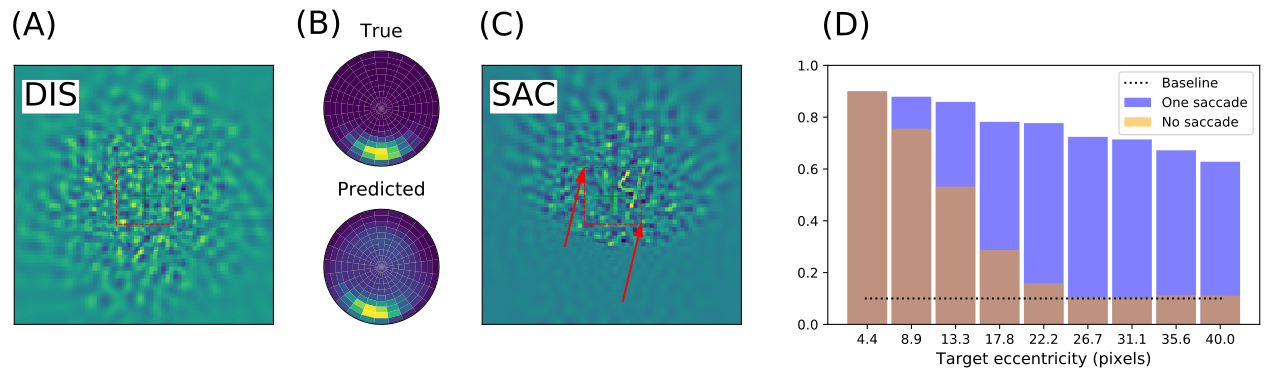
\includegraphics[width=\linewidth]{fig_result_robust.png}}
% 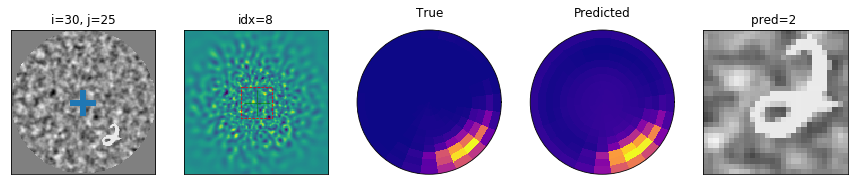
\includegraphics[]{../../2019-07-15_CNS/figures/CNS-saccade-8.png} % TRUE
\caption{
{\bf Simulated active vision agent}:
\A The visual display (\DIS , see also Figure~\ref{fig:intro}-C) is transformed into a retinotopic representation which is used as the input to the multi-layer neural network implementing the ``where'' pathway that predicts the accuracy map from the retinal image. %
\B We show after training the ``where'' pathway the network output ('Predicted') as compared with the ground truth ('True'). %
\C The network's output allows to generate a saccade to the most likely target position in visual space and to recenter the retinotopic map after a saccade (\SAC ), making possible to classify the digit on the central snippet. %
\D The active vision agent is tested at different eccentricities (in pixels) to estimate a final classification rate. Orange bars: accuracy of a central classifier ('No saccade') with respect to the target's eccentricity, averaged over 1,000 trials per eccentricity scale. Blue bars: Final classification rate after one saccade predicted by the ``Where'' pathway. % \if 0\ICANN{\color{blue} TODO: show three levels of noise Low (0.5) median (1.2) high (2). TODO: compare with Accuracy max (knowing the position)}\fi
\label{fig:results}}%
\end{figure}%
%%------------------------------%
%=================================================================
\subsection{Inferring where to look}
%=================================================================
After training the network, we evaluated simulations of the final accuracy at the landing of the predicted saccade (see Figure~\ref{fig:results}). For each different visual display (a different digit at a different position with a different noise clutter), a retinocentric visual input is processed (figure \ref{fig:results}-A), providing a predicted accuracy map (figure \ref{fig:results}-B) that can be compared to the actual future accuracy. Then, a saccade is carried out based on the most probable position as computed from the predicted accuracy map (figure \ref{fig:results}-C), and the final accuracy is computed from the ``what'' pathway using LeNet model. We observed that either the detection of the object's position was correct, thus allowing a classification proportional to the accuracy of the ``what'' pathway, either that the predicted accuracy map was wrong and generated a wrong classification with an accuracy at chance level. 
This process is repeated $1,000$ times for each different eccentricity, and the final average accuracy is shown as blue bars on figure \ref{fig:results}-D. It is compared to a central classifier trying to predict the category without doing a saccade (orange bars). As expected, the accuracy decreases with the eccentricity, for the targets become less and less visible in the periphery. The decrease is very rapid in the central classifier case: the accuracy drops to the baseline level
approximately at a pixel radius of $20$ around the center of fixation. In contrast, issuing a saccade is beneficial in up to the border of the image, thus allowing for a full covering of the initial image with an average accuracy of approximately $80\%$. The difference between the two distributions forms an ``accuracy gain'', that quantifies the benefit of active inference with respect to a central prior, interpreted as the information gain provided by the ``Where'' pathway.
% energy consumption

As our saccade selection algorithm may implement the essential operations done in the ``Where'' pathway, the central classifier may also reflect the response of the ``What'' pathway, giving the potential category of the digit. It is therefore possible to compare the two accuracy estimates to chose the most appropriate action: it may be that the accuracy is best in the ``What'' pathway and in that case no saccade is produced. The decision frontier lies between the first and the second spatial scale, allowing to pursue micro-saccades in the close vicinity of the target (2-3 pixels), in order to achieve a perfect centering.  In the other decision case, the ''What'' accuracy can still be considered to update the ``Where'' accuracy. When extending our framework to several saccades, this would allow in particular to ``explain away" the current position of the fixation and the neighboring ones. Such heuristic gives a principled formulation of the inhibition of return mechanism which is an important aspect for modeling saccades~\citep{Itti01}. In particular, we predict that such a mechanism is dependent on the class of inputs, and would be different for searching for faces as compared to digits. 

\subsection{Quantitative role of parameters}
%: effect of contrast
To test the robustness of our framework, we repeated the same experiment at different signal-to-noise ratios (SNR) of the input images. Indeed, there is an interdependence of both pathways, and it is crucial to 
The result of Figure~\ref{fig:results}-D, correspond to a SNR of $0.7$ and we replicated the result for SNRs of $0.3$ and $0.5$. First, we re-iterated for each SNR the whole process, first by learning the ``what'' pathway, then the accuracy maps and finally the ``where'' pathway. We first observed that the accuracy map was scaled in the ``what'' pathway by the maximal accuracy (at the center of the image), respectively at a value of approximately $53\%$, $82\%$ and $92\%$ for SNRs of $0.3$, $0.5$ and $0.7$. Then, we observed that behavior of the ``where'' pathway was similar at the different SNRs values, yet with the scaling imposed by the ``what'' pathway. This shows the robustness of our framework to different levels of noise.

%: scanning of other parameters
In addition, we controlled that these results are robust to changes in experimental or network parameters (see Figure~\ref{fig:params}). From the scan of all these parameters, the following observations were remarkable. First we verified that accuracy decreased when\texttt{noise} increased and while the bandwidth of the noise ($B_{sf}$) imported weakly, the spatial frequency of the noise was an important factor. In particular, final accuracy was worst for $\texttt{sf\_0} \approx 0.07$, that is when the characteristic textures elements was closest to the characteristic size of the objects. Second, we saw that the dimension of the ``where'' network was optimal for a dimensionality similar to that of the input but that this mattered weakly. More importantly was the dimensionality of the log-polar map, which proved that an optimal accuracy was achieved when using a number of $24$ of azimuthal directions in our experimental setting. Indeed, a finer log-polar grid requires more epochs to converge and may result in an over-fitting phenomenon hindering the final accuracy. Such fine tuning of paramemeters may prove to be important in practical applications and to optimize the compromise between accuracy and compression. 
%=================================================================
%------------------------------%
%: see Figure~\ref{fig:params}
\begin{figure}[t!]%%[p!]
\centering{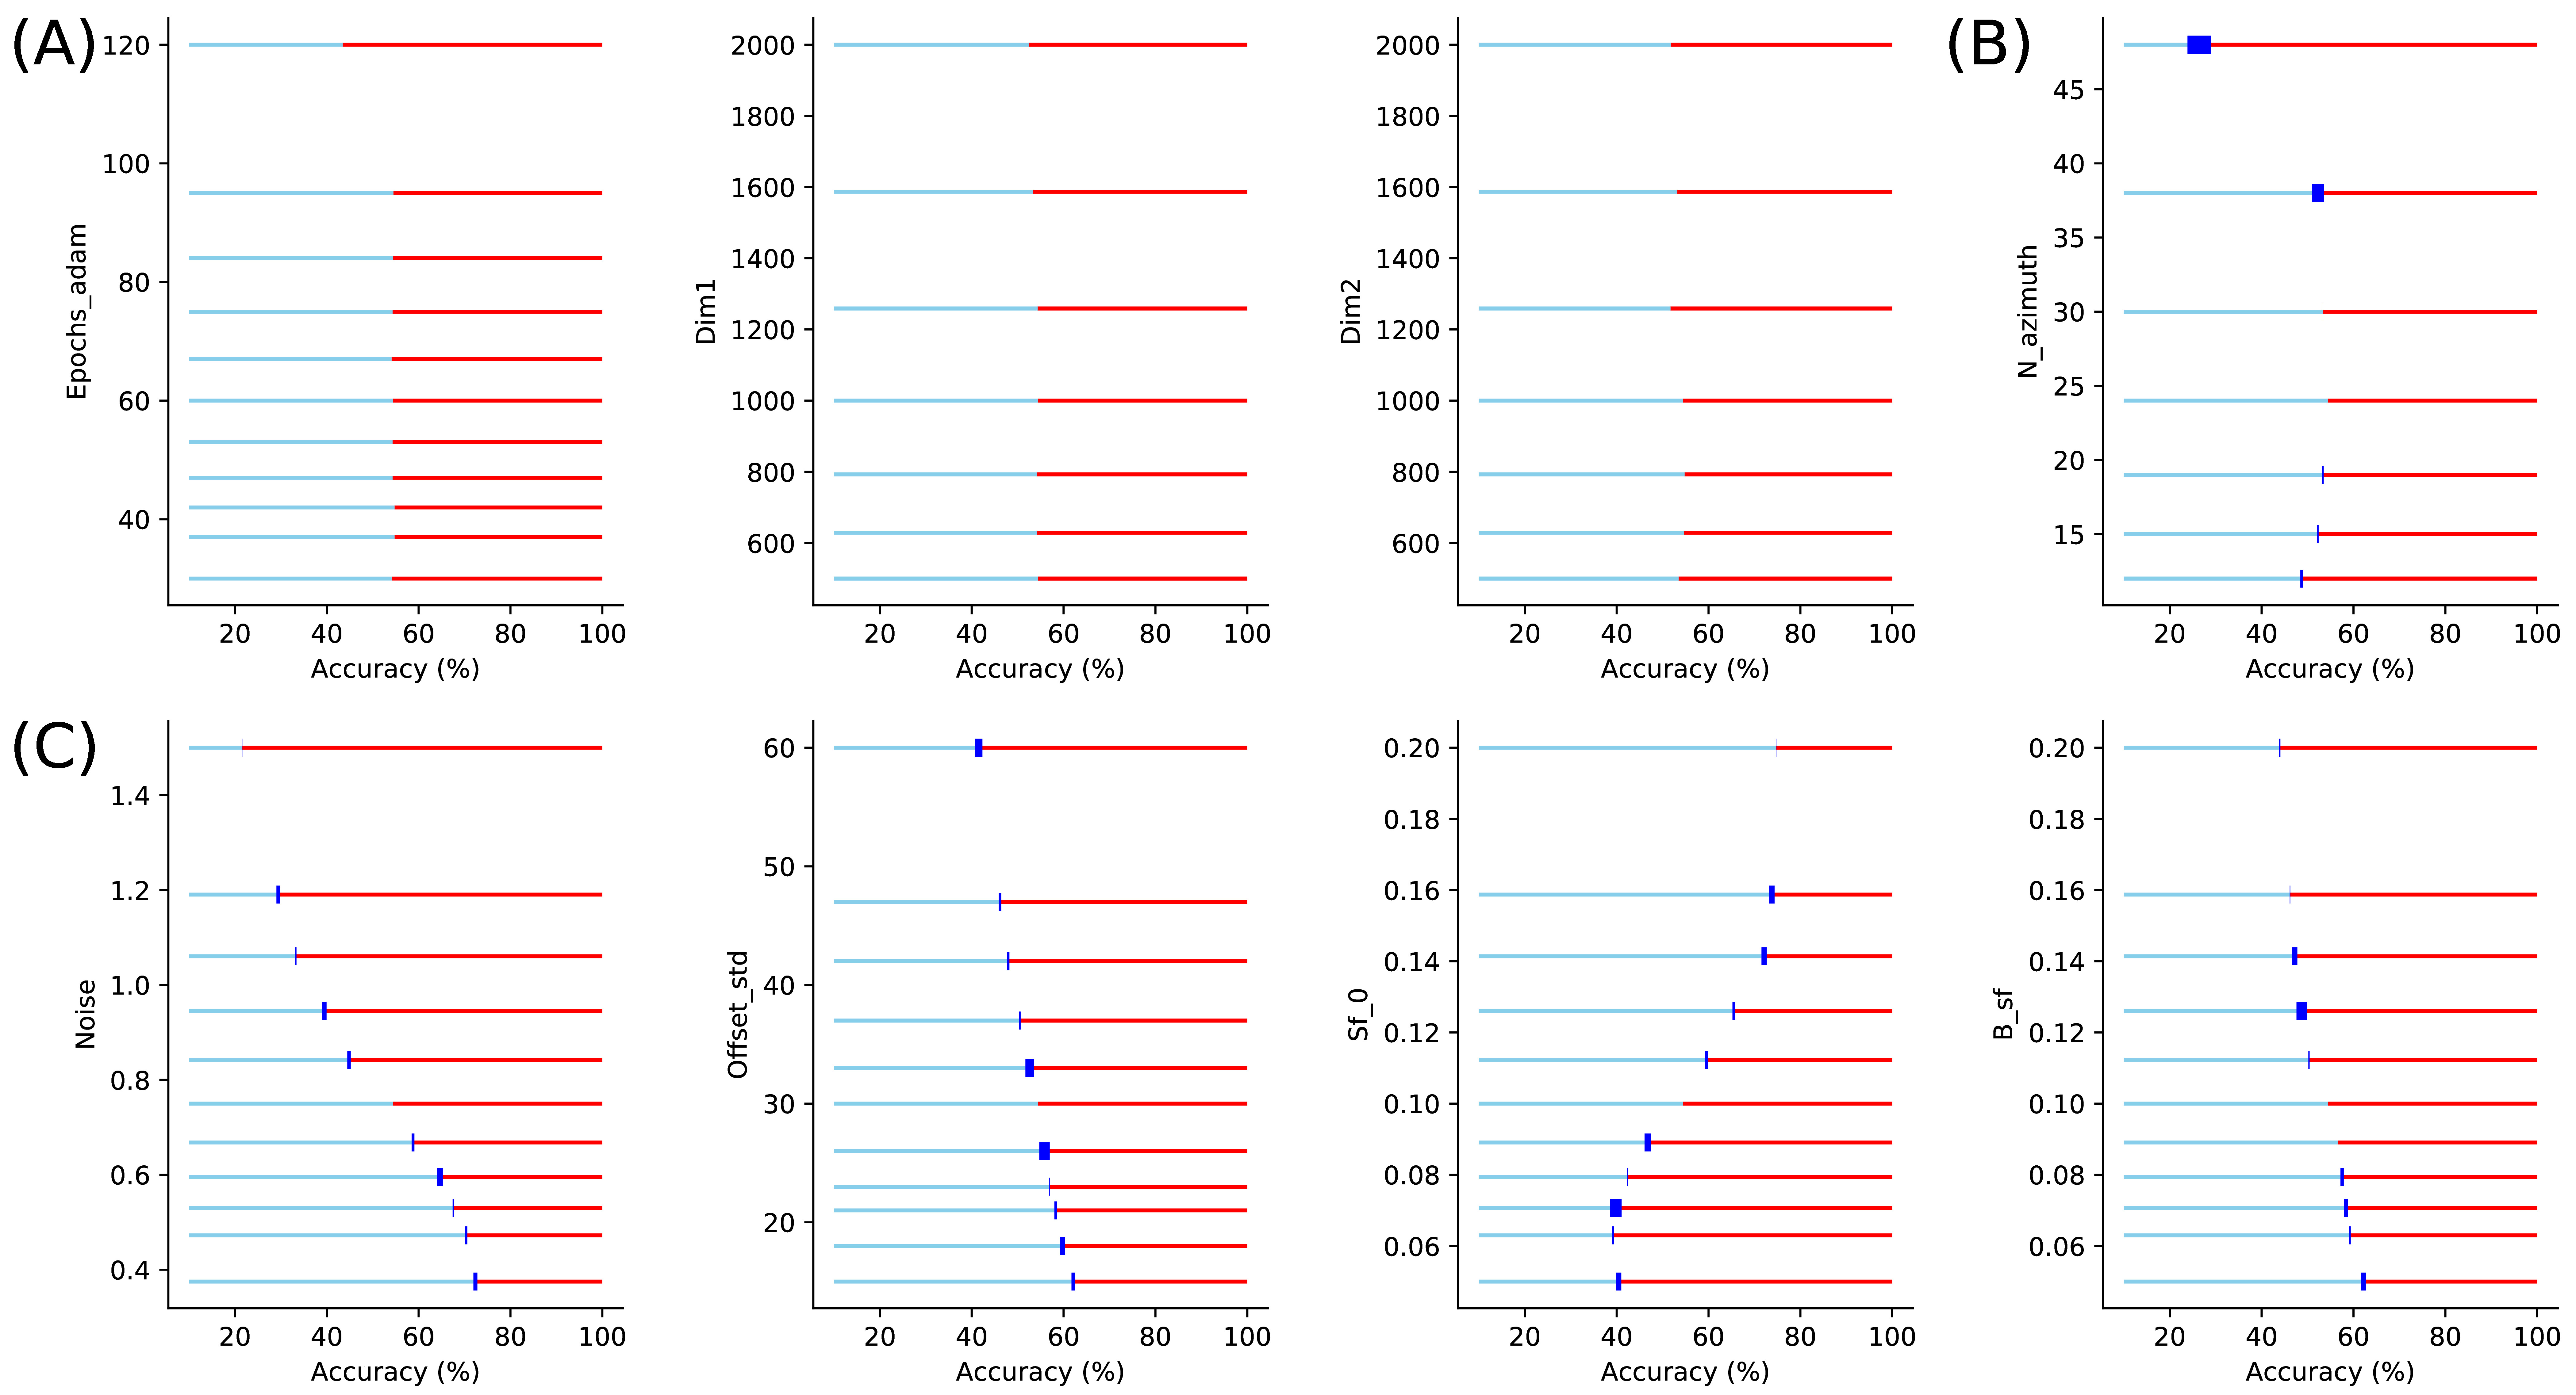
\includegraphics[width=\linewidth]{fig_params}}
\caption{
{\bf Quantitative role of parameters}: We show here variations of the average accuracy as a function of some free parameters of the model. All parameters of the presented model were tested, from the architecture of image generation, to the parameters of the neural network implementing the ``Where'' pathway (including meta-parameters of the learning paradigm). We show here the results which show the most significative impact on average accuracy. %
\A First, we tested some properties of the input, respectively from left to right: noise level (\texttt{noise}), mean spatial frequency of clutter \texttt{sf\_0} and bandwidth \texttt{B\_sf} of the clutter noise. This shows that average accuracy evolves with noise (see also Figure~\ref{fig:results} for an evolution as a function of eccentricity), but also to the characteristics of the noise clutter. In particular, there is a drop in accuracy whenever noise is of similar wavelength as digits, but which becomes less pronounced as the bandwidth increases. %
\B The accuracy also changes with the architecture of the foveated input as shown here by changing the number \texttt{N\_azimuth} of azimuth directions which are sampled in visual space. This shows a compromise between a rough azimuth representation and a large precision, which necessitates a longer training phase, such that the optimal number is around $20$ azimuth directions. %
\C Finally, we scanned parameters of the Deep Learning neural network. It shows that accuracy quickly converged after a characteristic time of approximately $25$ \texttt{epochs}. We then tested different values for the dimension of respectively the first (\texttt{dim1}) and second (\texttt{dim2}) hidden layers, showing weak changes in accuracy. %
\label{fig:params}}%
\end{figure}%
%%------------------------------%


% TODO : make a (minimal) psychophysics experiment= show an image as in figure 1, then in (ANS), make a 2AFC task by showing the true versus a random one -> web experiment using pavlovia?
